%%%%%%%%%%%%%%%%%%%%%%%%%%%%%%%%%%%%%%%%%%%%%%%%%%%%%%%%%%%%%%%%%%%%%%%%%%%%%%%%%%%%%%%%%%%%%%%%%%%%%%%%%%%%%%%%%%%%%%%%%%%%%%%%%%%%%%%%%%%%%%%%%%%%%%%%%%%%%%%%%%%%%%%
%%%%%%%%%%%%%%%%%%%%%%%%%%%%%%%%%%%%%%%%%%%%%%%%%%%%%%%%%%%%%%%%%%%%%%%%%%%%%%%%%%%%%%%%%%%%%%%%%%%%%%%%%%%%%%%%%%%%%%%%%%%%%%%%%%%%%%%%%%%%%%%%%%%%%%%%%%%%%%%%%%%%%%%
%%%%%%%%%%%%%%%%%%%%%%%%%%%%%%%%%%%%%%%%%%%%%%%%%%%%%%%%%%%%%%%%%%%%%%%%%%%%%%%%%%%%%%%%%%%%%%%%%%%%%%%%%%%%%%%%%%%%%%%%%%%%%%%%%%%%%%%%%%%%%%%%%%%%%%%%%%%%%%%%%%%%%%%

\FloatBarrier
\chapter{Simulated samples}
\label{ch:SimulatedSamples}

In order to design the search and to study background and signal characteristics, this analysis relies on simulated  SM and SUSY datasets.
An introduction to the techniques and tools required for the simulation of SM and beyond SM processes can be found in Section~\ref{ch:SimulationOfEvents}.

The following two sections present an overview of the SM (Section~\ref{sec:SMSamples}) and SUSY samples (Section~\ref{sec:SignalSamples}) used in this search.
All samples are reweighted to match the measured distribution of pileup interactions per event in data.
Additionally, event weights are applied to ensure the same ISR spectrum in simulation as in data.

%%%%%%%%%%%%%%%%%%%%%%%%%%%%%%%%%%%%%%%%%%%%%%%%%%%%%%%%%%%%%%%%%%%%%%%%%%%%%%%%%%%%%%%%%%%%%%%%%%%%%%%%%%%%%%%%%%%%%%%%%%%%%%%%%%%%%%%%%%%%%%%%%%%%%%%%%%%%%%%%%%%%%%%
\section{Standard Model background samples}
\label{sec:SMSamples}
To investigate the sources of background, various simulated SM samples are used.
Since this analysis aims at making use of \dedx, a data format is required that includes tracker hit information, the so-called RECO format~\cite{bib:DataFormats}.
Unfortunately, not all SM processes are available in this format making it impossible to compare the total number of events in simulation and data.
This, however, does not constitute a serious problem since this analysis will finally use data-based background estimation methods.
The simulated SM datasets can still be used to compare the shapes of important distributions in simulation and data.\footnote{For example, the simulated \ZInvJets sample that can contribute to the background of this search via fake tracks is not available in RECO format. However, as the shape of important observables of fake tracks is independent of the underlying process, this background can be studied with a simulated \WJets sample.}
Still, the most important SM background sample including \WJets events is available.
Due to the intrinsic missing energy in \WJets events it constitutes the major background to the presented search (see Section~\ref{ch:BackgroundEstimation} for further details on the backgrounds). \\

In Table \ref{tab:SMsamples_RECO} all available SM samples used in this analysis are listed.
The matrix-elements of the \WJets, \ttbarJets and \ZlepJets samples are generated using \madgraph5~\cite{bib:Madgraph_2014}. 
For the QCD sample \pythiaSix~\cite{bib:Pyhtia6_2006} is used for generation.
All samples are then passed to \pythia6 to simulate the hadronisation and the showering. %, the underlying event and the beam remnants.
The interactions between the particles and the detector material is simulated using \geant~\cite{bib:Geant4_2003,bib:Geant4_2006}.

Due to the size of the samples (between 5 and 70\,TB per sample) a reduction is required in order to limit the storage space requirements.
This is achieved by selecting only events which contain at least one jet with a minimum transverse momentum of $\pt>60\gev$.

In addition, further simulated samples not containing \dedx information are used (so-called AOD samples).
Because of their much smaller size, these samples are available in full size.
They are needed to study the background inclusively in the variable \dedx.

\renewcommand{\arraystretch}{1.5}
\begin{table}[!h]
\centering
\caption{Available Standard Model background samples containing $\Delta E/\Delta x$ information that are used for background estimation studies.}
\label{tab:SMsamples_RECO}
\makebox[0.99\textwidth]{
\begin{tabular}{llll}
\multicolumn{4}{c}{} \\
\toprule
 Process & Generator & Cross section $\left[\pb\right]$ & $\mathcal{O}_{\text{calculation}}^{\text{cross section}}$ \\%& Size $\left[\text{TB}\right]$\\
\midrule
 \WJets                                        &   \madgraph5     &  36703.2      &  NNLO \cite{bib:FEWZ} \\%& 70.4 \\
 \ttbarJets                                    &   \madgraph5     &  245.8        &  NNLO \cite{bib:ttbar:Czakon_2013}\\%& 55.9 \\
 \ZlepJets ($\ell=e,\mu,\tau$)                 &   \madgraph5     &  3531.9       &  NNLO \cite{bib:FEWZ} \\%& 5.1  \\
 QCD ($50\gev<\hat{p}_{\text{T}}<1400\gev$)      &   \pythia6      &  9374794.2    &  LO  \\%% & 44.3\\
\bottomrule
%\multicolumn{4}{c}{} 
\end{tabular}}
\end{table}  

%%%%%%%%%%%%%%%%%%%%%%%%%%%%%%%%%%%%%%%%%%%%%%%%%%%%%%%%%%%%%%%%%%%%%%%%%%%%%%%%%%%%%%%%%%%%%%%%%%%%%%%%%%%%%%%%%%%%%%%%%%%%%%%%%%%%%%%%%%%%%%%%%%%%%%%%%%%%%%%%%%%%%%%
\section{Signal samples}
\label{sec:SignalSamples}
For the investigation of a possible SUSY signal, events containing either chargino pair production $q\bar{q} \rightarrow \chipm \chimp$ or chargino neutralino production $q\bar{q} \rightarrow \chipm \chiO$ are simulated within this thesis. 
The simulation of the samples is done as described in Section~\ref{sec:SMSamples} for the \WJets sample.
However, a special treatment for long-lived particles is required for this analysis.
In order to get a correct detector simulation of the energy loss of long-lived particles that decay after the beam pipe, the decay of the chargino cannot be simulated within \madgraph or \pythia but needs to be simulated within \geant.
The decay mode of the chargino is also specified within \geant to a neutralino plus pion decay, $ \chipm \rightarrow \chiO\, \pi^{\pm}$.

To reduce the required computing resources, the simulation is only done for a few lifetimes (\ctau = 1\cm, 5\cm, 10\cm, 50\cm, 100\cm, 1\,000\cm and 10\,000\cm).
The lifetime is hereby not controlled by changing the mass gap between the chargino and the neutralino but is independently specified within \geant.
In order to scan in a high resolution over the lifetime space, other lifetimes are generated using lifetime reweighting.
The weight for each event depends on the individual proper lifetime of the chargino and is given by
\begin{equation}
w = \prod_{i=1}^n \frac{\tau^{\text{gen}}}{\tau^{\text{target}}}\cdot  \exp \left[ t_i \cdot \left( \frac{1}{\tau^{\text{gen}}} - \frac{1}{\tau^{\text{target}}} \right) \right] ,
\end{equation}
where $n$ is the  number of charginos in the event, $\tau^{\text{gen}}$ is the generated mean lifetime in the particle rest frame and $t_i$ is the individual proper lifetime of the chargino. 
The targeted mean lifetime is given by $\tau^{\text{target}}$. 
A derivation of this formula can be found in Appendix~\ref{app:LifetimeReweighting}.
Using this reweighting procedure a good coverage of the lifetime space can be achieved with lifetimes of $1\cm \leq \ctau \leq 10^4 \cm $. %\ctau = $a\cdot10^{n}$ for $n=0,1,2,3$ and $a=\left[1,9\right]$.
Figure~\ref{fig:LifetimeReweighting} shows the exponential distribution of the individual proper lifetime of the charginos after the reweighting of a simulated sample with $c\tau^{\text{gen}}=50\cm$ to a lifetime of $c\tau^{\text{target}}=10\cm$.
\begin{figure}[!b]
  \centering 
  \begin{tabular}{c}
    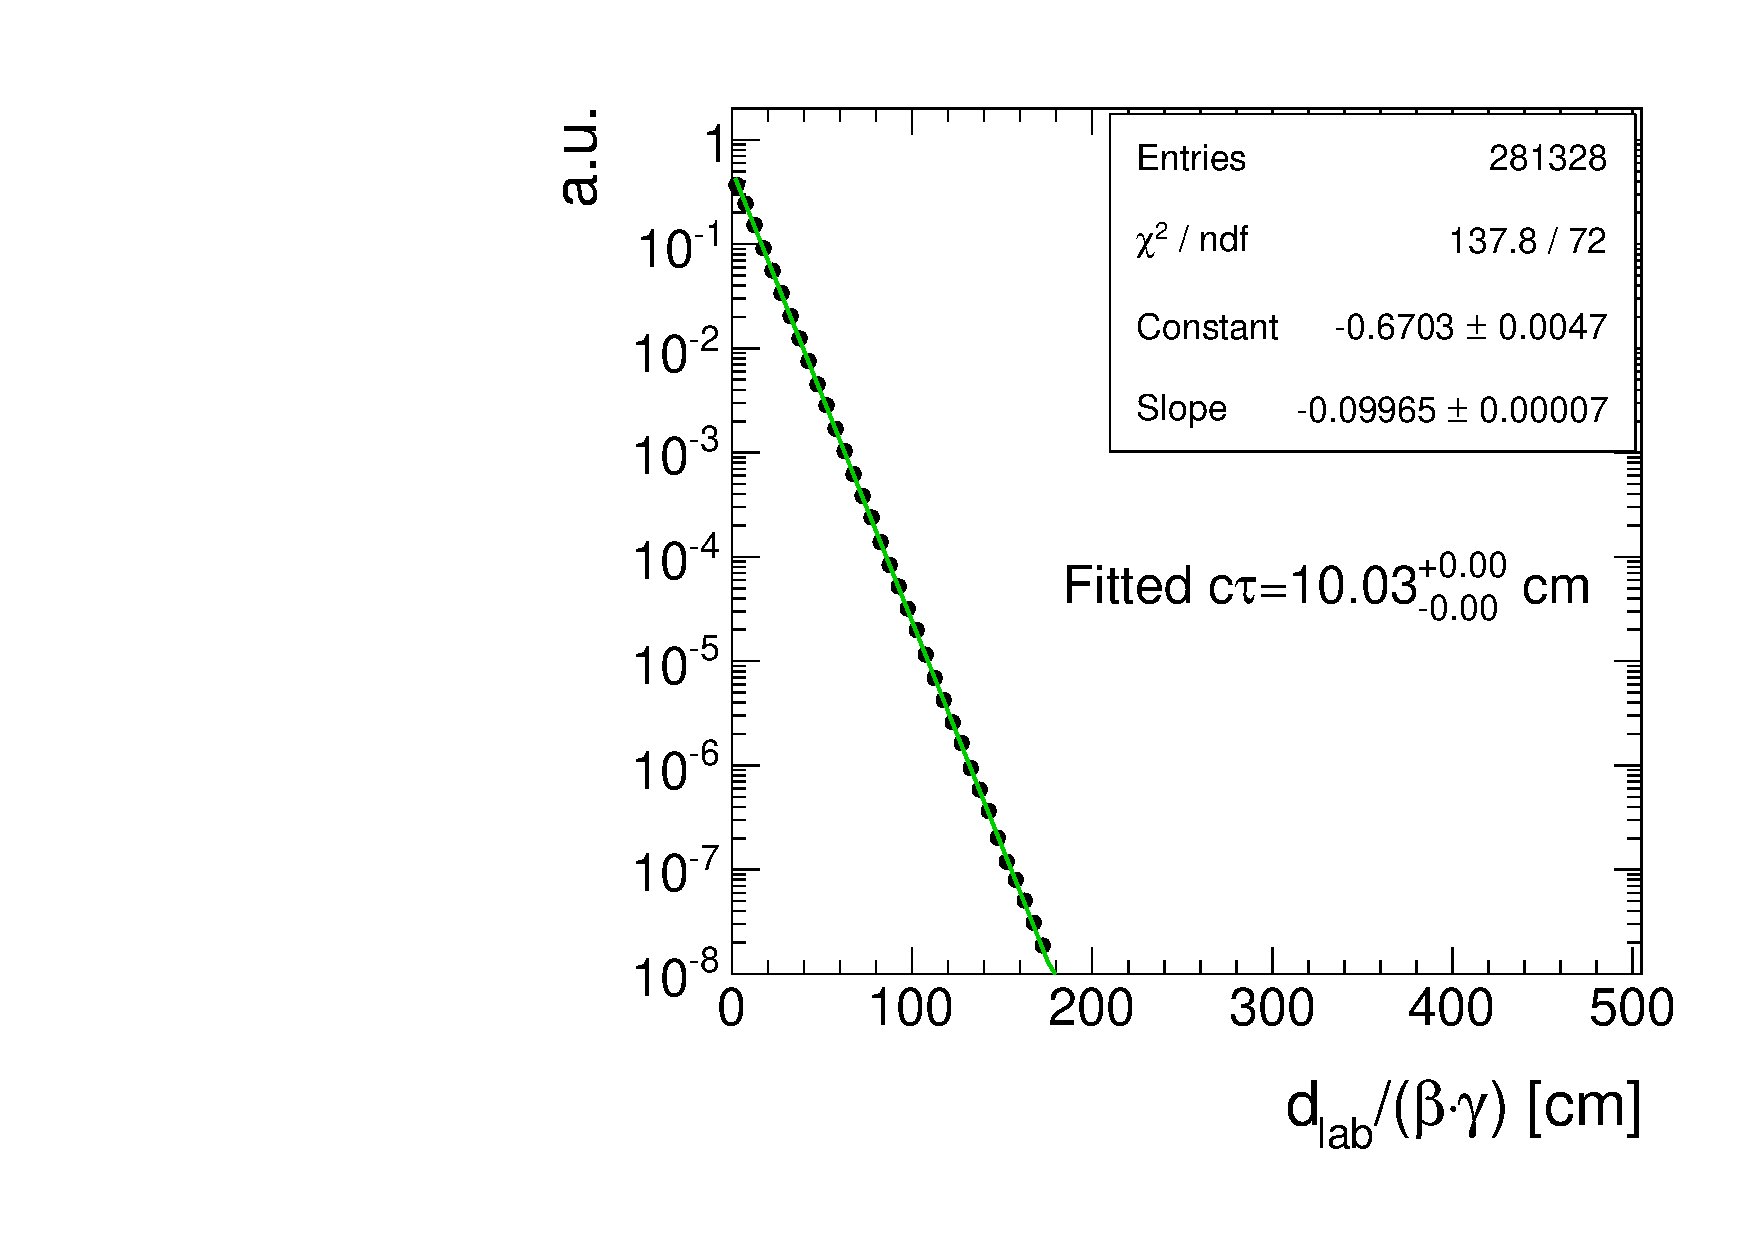
\includegraphics[width=0.49\textwidth]{figures/analysis/Samples/10cm.pdf}
  \end{tabular}
  \caption{Normalised distribution of the proper individual lifetime $d_{\text{lab}}/\left(\beta\gamma \right)$ of all charginos contained in a signal sample with a generated lifetime of $c\tau^{\text{gen}}=50\cm$ reweighted to a lifetime of $c\tau^{\text{target}}=10\cm$. Fitting an exponential curve $a\cdot \exp\left[\frac{1}{c \tau } c t_i\right]$ yields $c\tau=\text{slope}^{-1}=10\cm$.}
  \label{fig:LifetimeReweighting}
\end{figure}
It can be seen that the reweighting procedure does indeed reproduce the targeted lifetime of 10\cm.


All samples are generated for different masses of the chargino, but always almost mass-degenerate to the lightest neutralino.
The mass gap between chargino and neutralino is set to 150\mev and, as said before, is hereby disentangled to the chargino lifetime for the simulation of the signal samples.
However, since this analysis does not make use of the decay products of the chargino and the mass gap is for all simulated lifetimes of a similar small size, the choice of the mass gap does not affect the signal prediction.
Six different masses from 100\gev to 600\gev are simulated.
This leads to a total number of 42 signal samples.
In Table~\ref{tab:SignalCrossSections}, the cross sections at $\sqrt{s}=8\tev$ for $\chipm\chimp$ and $\chipm\chiO$ production for wino-like charginos and neutralinos are listed~\cite{bib:SignalCrossSection_2012,bib:SignalCrossSection_2013}.
The cross section does not depend on the lifetime of the chargino.
\renewcommand{\arraystretch}{1.5}
\begin{table}[h]
\centering
\caption{Simulated signal mass points with corresponding cross sections at NLO-NLL (NLO: next-to-leading order, NLL: next-to-leading logarithmic) accuracy for wino-like charginos~\cite{bib:SignalCrossSection_2012,bib:SignalCrossSection_2013}.}
\label{tab:SignalCrossSections}
\makebox[0.99\textwidth]{
\begin{tabular}{lll}
\multicolumn{3}{c}{} \\
\toprule
 $m_{\chipm}\left[\gev\right]$ & $\sigma_{\chipm\chimp}\left[\pb\right]$  & $\sigma_{\chiO\chimp}\left[\pb\right]$ \\
\midrule
 100     &  5.8234     &  11.5132 \\
 200     &  0.37924    &  0.77661 \\
 300     &  0.06751    &  0.14176 \\
 400     &  0.01751    &  0.03758 \\
 500     &  0.00553    &  0.01205 \\
 600     &  0.00196    &  0.00431 \\
\bottomrule
%\multicolumn{3}{c}{} 
\end{tabular}}
\end{table}  

%%%%%%%%%%%%%%%%%%%%%%%%%%%%%%%%%%%%%%%%%%%%%%%%%%%%%%%%%%%%%%%%%%%%%%%%%%%%%%%%%%%%%%%%%%%%%%%%%%%%%%%%%%%%%%%%%%%%%%%%%%%%%%%%%%%%%%%%%%%%%%%%%%%%%%%%%%%%%%%%%%%%%%%%%%%%%%%%%%%%
%%%%%%%%%%%%%%%%%%%%%%%%%%%%%%%%%%%%%%%%%%%%%%%%%%%%%%%%%%%%%%%%%%%%%%%%%%%%%%%%%%%%%%%%%%%%%%%%%%%%%%%%%%%%%%%%%%%%%%%%%%%%%%%%%%%%%%%%%%%%%%%%%%%%%%%%%%%%%%%%%%%%%%%%%%%%%%%%%%%%
